\chapter{Código sistema de usuários}

Neste apêndice encontram-se algumas partes importantes do código do Sistema de Usuários. O código inteiro pode ser baixado no \textit{link}: \url{https://github.com/CamiloAvelar/user-service}

\begin{lstlisting}[caption=Exemplo do código do \textit{interactor} de criação do usuário]
import Interactor from './interactor';
import usersRep from '../repositories/users.rep';
import bcrypt from 'bcrypt';
import config from './../config/config';

class CreateUserBs extends Interactor {
	constructor(){
		super();
	}
	
	async execute({ name, password, allowedBathTime }) {
	
		if (!allowedBathTime) {
			allowedBathTime = 10;
		}
	
		const hash = await bcrypt.hash(password.toString(), config.bcrypt.saltRounds);
	
		const user = await usersRep.createUser({ name, password: hash, allowedBathTime });
		
		if(!user) {
			throw 'Nao foi possivel criar o usuario!';
		}
		
		const response = {
			id: user.user_id,
			name: user.user.name,
			allowed_bath_time: user.allowed_bath_time,
		};
		
		return response;
	}
}

export default CreateUserBs;
\end{lstlisting}

\begin{lstlisting}[caption=Exemplo do código do \textit{interactor} de edição de senha de usuários]
import Interactor from './interactor';
import usersRep from '../repositories/users.rep';
import bcrypt from 'bcrypt';
import config from './../config/config';

class EditPasswordBs extends Interactor {
	constructor(){
		super();
	}
	
	async execute({ id, new_password }) {
	
		const hash = await bcrypt.hash(new_password.toString(), config.bcrypt.saltRounds);
		
		const editedUser = await usersRep.editPassword({ id, password: hash });
		
		const response = editedUser[0] === 1 ? {
			status: 200,
			message: 'Usuario editado com sucesso'
		} : 
		{
			status: 500,
			message: 'Erro ao editar usuario'
		};
		
		return response;
	}
}
\end{lstlisting}

\newpage

\begin{lstlisting}[caption=Exemplo do código do \textit{interactor} de edição de tempo de banho dos usuários]
import Interactor from './interactor';
import usersRep from '../repositories/users.rep';

class EditUserTimeBs extends Interactor {
	constructor() {
		super();
	}
	
	async execute({ id, new_time }) {
	
		const editedUser = await usersRep.editUserTime({ id, new_time });
		
		const response = editedUser[0] === 1 ? {
			status: 200,
			message: 'Usuario editado com sucesso'
		} : 
		{
			status: 500,
			message: 'Erro ao editar usuario'
		};
		
		return response;
	
	}
}
\end{lstlisting}

\newpage

\begin{lstlisting}[caption=Exemplo do código do \textit{interactor} de autorização de usuários]
import Interactor from './interactor';
import usersRep from '../repositories/users.rep';
import bcrypt from 'bcrypt';

class AuthorizeUserBs extends Interactor {
	constructor(){
		super();
	}
	
	async execute({ id, pass }) {
		const user = await usersRep.getUser({ id });
		
		if(!user) {
			throw {error: 'Usuario nao encontrado'};
		}
		
		const match = await bcrypt.compare(pass.toString(), user.password);
		
		return {
			allowed: match
		};
	}
}
\end{lstlisting}

\newpage

\begin{lstlisting}[caption=Exemplo do código do \textit{interactor} de cadastro de banhos]
import Interactor from './interactor';
import bathsRep from '../repositories/baths.rep';

class BathsBs extends Interactor {
	constructor(){
		super();
	}
	
	async execute({ user_id, bath_time }) {
	
		const bath = await bathsRep.createBath({
			user_id,
			bath_time
		});
		
		if(!bath) {
			throw 'Nao foi possivel cadastrar o banho';
		}
		
		return bath;
		}
		
		async getBaths ({ user_id }) {
		
		const baths = await bathsRep.getBaths({
			user_id,
		});
		
		return baths;
	}
}

export default BathsBs;
\end{lstlisting}

\newpage

\begin{lstlisting}[caption=Exemplo do código do \textit{interactor} para recuperar informações dos usuários]
import Interactor from './interactor';
import usersRep from '../repositories/users.rep';

class GetUserBs extends Interactor{
	constructor(){
		super();
	}
	
	async execute({ id }) {
	const user = await usersRep.getUser({ id });
	
	if(!user) {
		throw {error: 'Nao foi possivel localizar o usuario!'};
	}
	
	const response = {
		id: user.id,
		name: user.name,
		allowedBathTime: user.user_setting.allowed_bath_time
	};
	
	return response;
	}
}
\end{lstlisting}

%\begin{figure}[htbp]
%	\centering
%	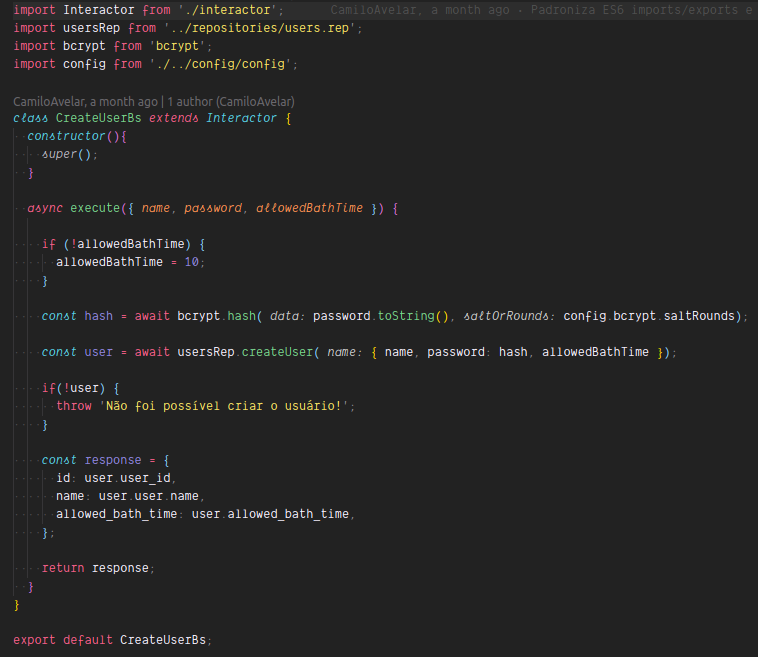
\includegraphics[width=1\linewidth]{figuras/userservice/createuser.png}
%	\caption{Código para criar usuário}
%	\label{fig:createuser}
%\end{figure}
%
%\begin{figure}[htbp]
%	\centering
%	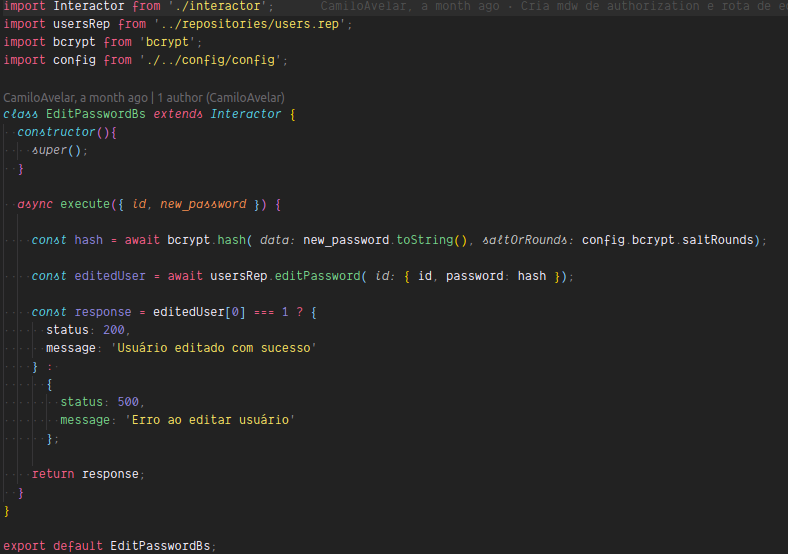
\includegraphics[width=1\linewidth]{figuras/userservice/editpassword.png}
%	\caption{Código para editar senha do usuário}
%	\label{fig:editpass}
%\end{figure}
%
%\begin{figure}[htbp]
%	\centering
%	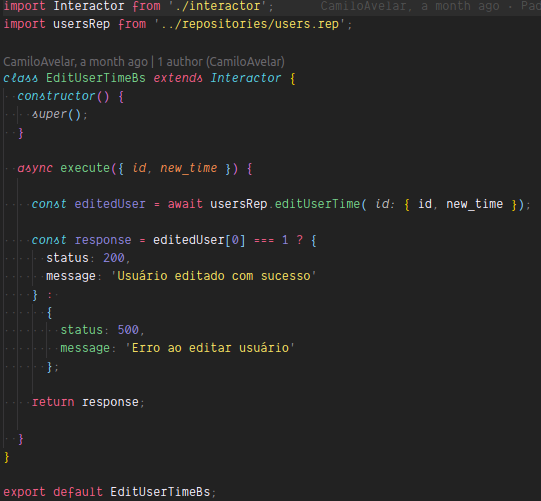
\includegraphics[width=1\linewidth]{figuras/userservice/edittime.png}
%	\caption{Código para editar tempo do usuário}
%	\label{fig:edittime}
%\end{figure}
%
%\begin{figure}[htbp]
%	\centering
%	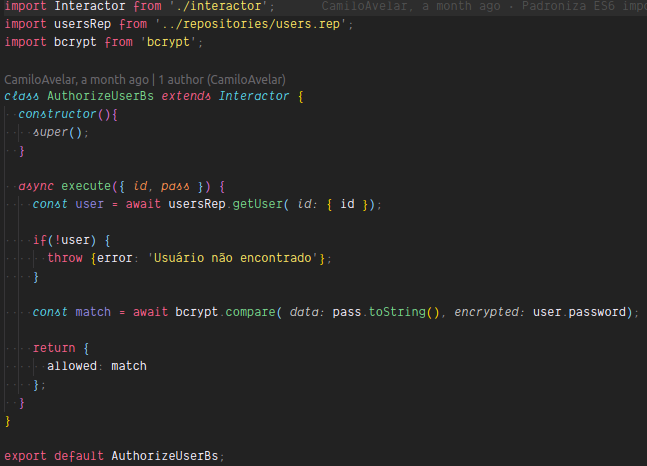
\includegraphics[width=1\linewidth]{figuras/userservice/authorizeuser.png}
%	\caption{Código para autorizar usuário}
%	\label{fig:autorizar}
%\end{figure}
%
%\begin{figure}[htbp]
%	\centering
%	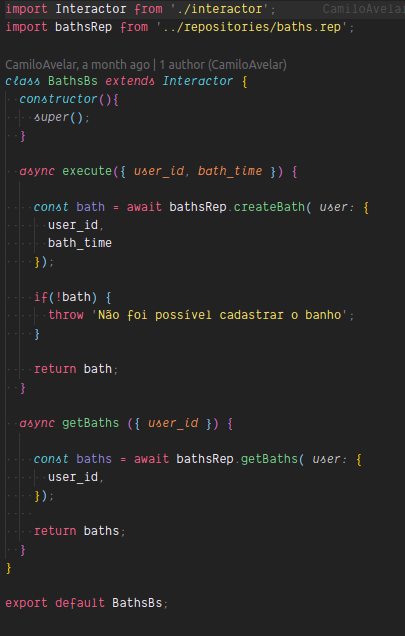
\includegraphics[width=1\linewidth]{figuras/userservice/baths.png}
%	\caption{Código para cadastrar banho do usuário}
%	\label{fig:cadastra-banho}
%\end{figure}
%
%\begin{figure}[htbp]
%	\centering
%	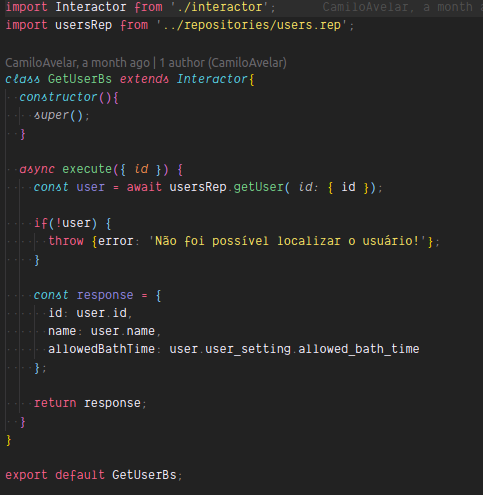
\includegraphics[width=1\linewidth]{figuras/userservice/getuser.png}
%	\caption{Código para recuperar usuários}
%	\label{fig:getuser}
%\end{figure}

\chapter{Código sistema de comunicação MQTT}

Neste apêndice encontram-se algumas partes importantes do código do Sistema de comunicação. O código inteiro pode ser baixado no \textit{link}: \url{https://github.com/CamiloAvelar/mqtt-logger-service}

\begin{lstlisting}[caption=Exemplo do código de comunicação MQTT]
const mqtt = require('mqtt');
const EventEmitter = require('events');


class MqttHandler extends EventEmitter {
	constructor() {
		super();
		this.mqttClient = null;
		this.host = 'mqtt://mosquitto';
		this.username = 'mqtt_user'; // mqtt credentials if these are needed to connect
		this.password = '100200300';
	}
	
	
	connect() {
		const self = this;
		this.mqttClient = mqtt.connect(this.host, { username: this.username, password: this.password });
		
		this.mqttClient.on('error', (err) => {
			console.log(err);
			this.mqttClient.end();
		});
		
		this.mqttClient.on('connect', () => {
			console.log(`mqtt client connected to ${this.host}`);
		});
		
		this.mqttClient.on('close', () => {
			console.log(`mqtt client disconnected`);
		});
		
		this.mqttClient.on('message', (topic, message) => {
			const builtMessage = {
				topic,
				message: message.toString()
			};
		
			self.emit('messageReceived', builtMessage);
		})
	}
	
	subscribe(topic) {
		this.mqttClient.subscribe(topic, {qos: 0});
	}
	
	sendMessage(message, topic) {
		this.mqttClient.publish(topic, message);
	}
}

module.exports = MqttHandler;
\end{lstlisting}

\begin{lstlisting}[caption=Exemplo do código responsável por lidar com informações do tempo de banho]
const requestService = require('./requestService');

class timeHandler {
	constructor(mqttClient) {
		this.mqttClient = mqttClient;
		this.allowedTime;
		this.interval;
		this.nowDate;
		this.endDate;
		this.userId;
	}
	
	countTime(allowedTime, id) {
		this.userId = id;
		this.allowedTime = allowedTime;
		this.nowDate = new Date();
		
		this.interval = setInterval(() => {
		this.mqttClient.sendMessage('stop', 'actuator');
		this.clearBathInterval();
		}, this.allowedTime);
	}
	
	async endTime() {
		this.clearBathInterval();
		this.endDate = new Date();
		
		const bathTime = this.endDate - this.nowDate;
		
		console.log('BATHTIME>>>', bathTime);
		await this._requestUserService(bathTime);
	}
	
	clearBathInterval(){
		clearInterval(this.interval);
	}
	
	async _requestUserService(time) {
		const requestOptions = {
			type: 'POST',
			endpoint: 'banho',
			body: {
			user_id: this.userId,
			bath_time: time
			},
		};
		
		return await requestService.userRequest(requestOptions);
	}
}

module.exports = timeHandler;
\end{lstlisting}

\newpage

\begin{lstlisting}[caption=Exemplo do código que lida com a comunicação com o InfluxDB]
const requestService = require('./requestService');

class KeysHandler {
	constructor(mqttClient) {
		this.keyBuffer = '';
		this.working = false;
		this.gettingPassword = false;
		this.userId;
		this.mqttClient = mqttClient;
	}
	
	async handle(message) {
		if(message === '*') {
			this.working = !this.working;
			this.gettingPassword = false;
			return;
		}
	
		if((this.working || this.gettingPassword) && message !== '#') {
			this.keyBuffer += message;
		}
		
		if(message === '#') {
			this.working = false;
			try {
				const response = await this._requestUserService();
				console.log(response);
				this.gettingPassword ? (response.allowed ? this.mqttClient.sendMessage('start', 'actuator') : console.log('NAO AUTORIZADO')) : 
				this.mqttClient.sendMessage(JSON.stringify(response), 'user');
				this.gettingPassword = !this.gettingPassword;
			} catch (err) {
				console.log(err.message)
			} finally {
				this.keyBuffer = '';
			}
		}
	}
	
	async _requestUserService() {
		const requestOptions = this.gettingPassword ? {
			type: 'POST',
			endpoint: `usuario/autorizar`,
			body:{
				id: this.userId,
				password: this.keyBuffer
			},
			}: {
				type: 'GET',
				endpoint: `usuario/${this.keyBuffer}`,
			body: null,
		};
		
		return requestService.userRequest(requestOptions)
		.then((response) => {
			this.userId = this.gettingPassword ? this.userId : response.id;
			return response
		}).catch(err => {throw err});
	}
}

module.exports = KeysHandler;
\end{lstlisting}

%\begin{figure}[htbp]
%	\centering
%	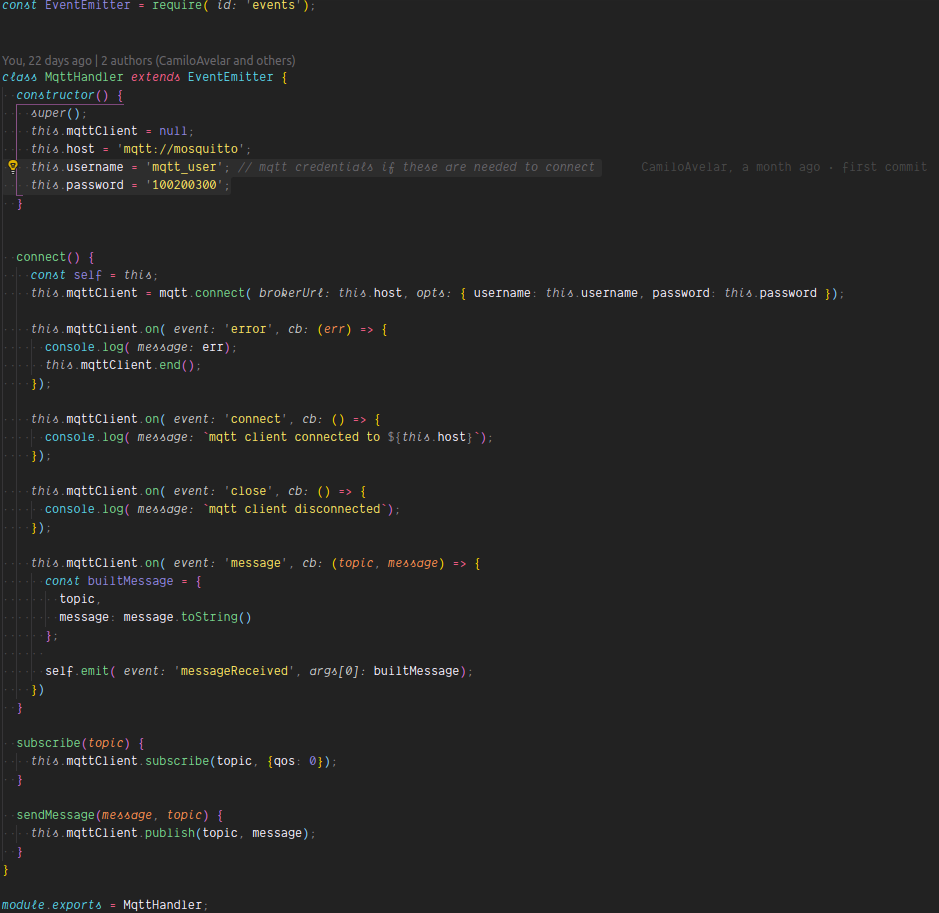
\includegraphics[width=1\linewidth]{figuras/mqttlogger/mqtt.png}
%	\caption{Código para comunicação mqtt}
%	\label{fig:mqtt}
%\end{figure}
%
%\begin{figure}[htbp]
%	\centering
%	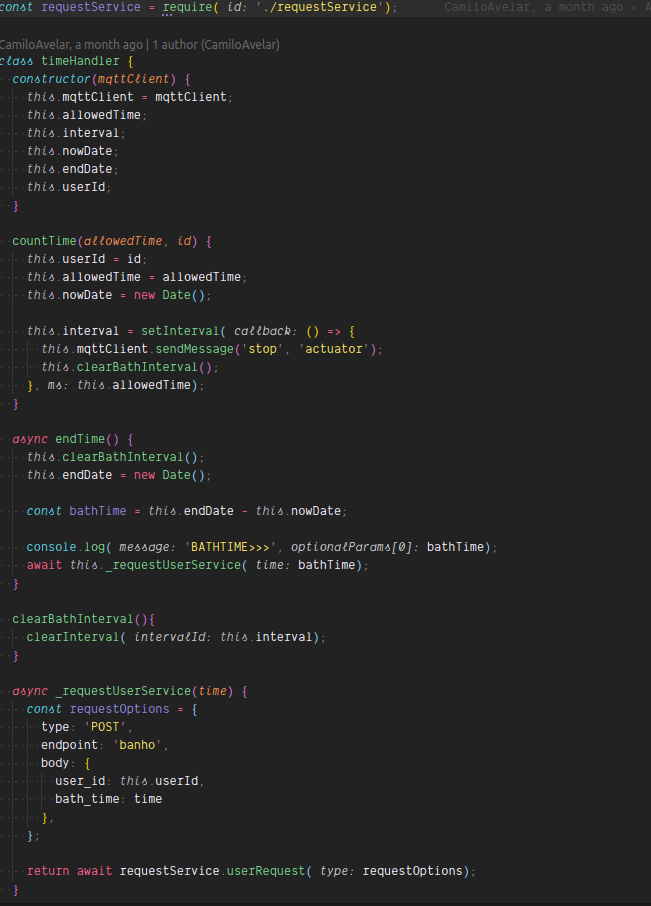
\includegraphics[width=1\linewidth]{figuras/mqttlogger/time.png}
%	\caption{Código que lida com o tempo do banho}
%	\label{fig:time}
%\end{figure}
%
%\begin{figure}[htbp]
%	\centering
%	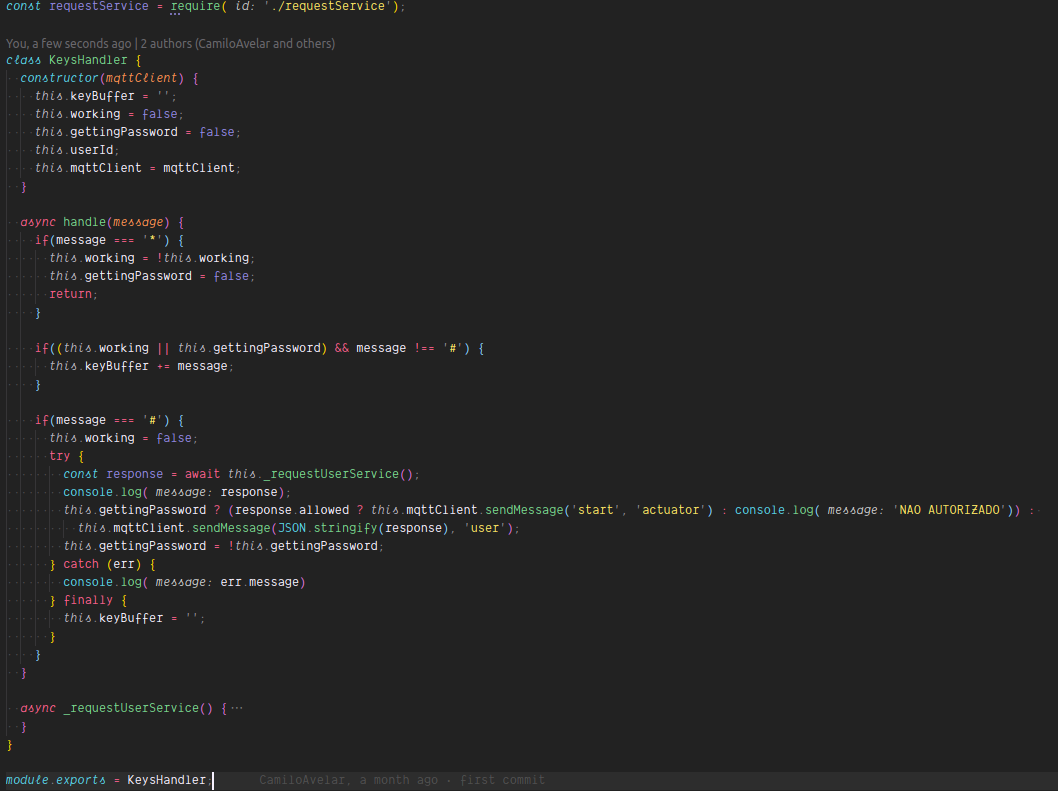
\includegraphics[width=1\linewidth]{figuras/mqttlogger/keystopic.png}
%	\caption{Código que lida com as teclas apertadas no teclado numérico}
%	\label{fig:keys}
%\end{figure}
%
%\begin{figure}[htbp]
%	\centering
%	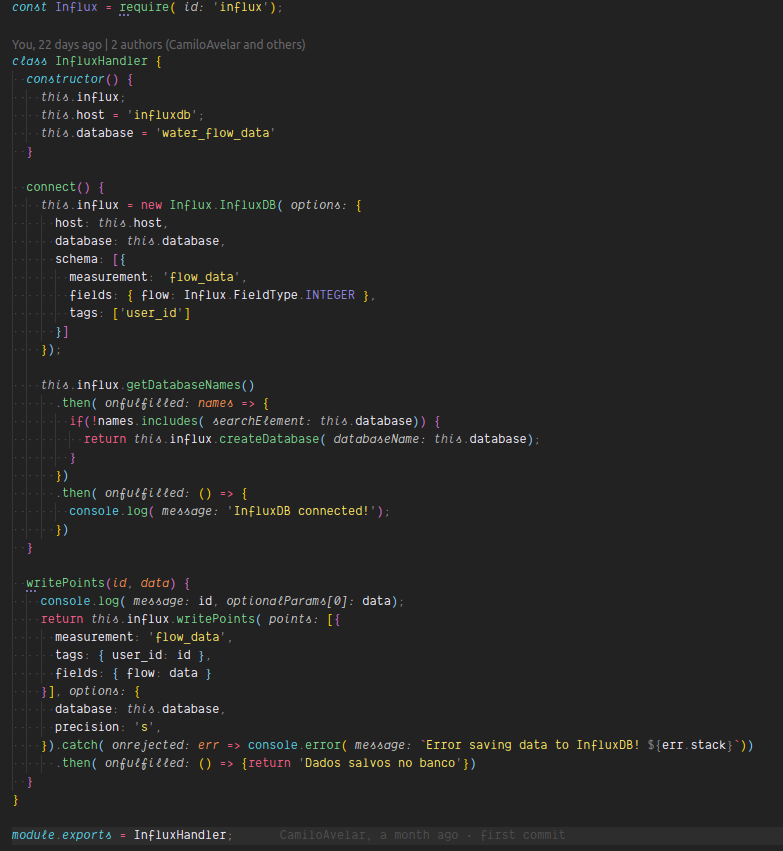
\includegraphics[width=1\linewidth]{figuras/mqttlogger/influx.png}
%	\caption{Código que lida com a comunicação com o InfluxDB}
%	\label{fig:influx}
%\end{figure}

%\chapter{Docker-compose.yml}
%
%\begin{lstlisting}[language=Python]
%version: "3.5"
%
%services:
%	user:
%		build: ./user-service
%		command: gulp
%		depends_on:
%			- postgres
%		volumes:
%			- ./user-service:/app
%		ports:
%			- "3001:3001"
%		networks:
%			- default
%
%	mqtt-logger:
%		build: ./mqtt-logger
%		command: npm start
%		depends_on:
%			- mosquitto
%		volumes:
%			- ./mqtt-logger:/app
%		ports:
%			- "3002:3002"
%
%	postgres:
%		image: postgres
%		restart: always
%		environment:
%		POSTGRES_USER: pi
%		POSTGRES_PASSWORD: 100200300
%		POSTGRES_DB: postgres
%		CONFIGS: "listen_addresses:'*'"
%		volumes:
%			- ./postgres/data:/var/lib/postgresql/data
%		expose:
%			- "5432"
%		ports:
%			- "5432:5432"
%		networks:
%			- default
%
%	migration:
%		image: src_user:latest
%		command: ["./wait-for-it/wait-for-it.sh", "postgres:5432", "--", "npm", "run", "migrate"]
%		links:
%			- postgres
%		depends_on:
%			- postgres
%
%	homeassistant:
%		container_name: homeassistant
%		restart: unless-stopped
%		image: homeassistant/home-assistant
%		volumes:
%			- ./homeassistant:/config
%		depends_on:
%			- mosquitto
%		network_mode: host
%		privileged: true
%		expose:
%			- "8123"
%		ports:
%			- "8123:8123"
%
%	influxdb:
%		image: influxdb:latest
%		container_name: influxdb
%		restart: always
%		ports:
%			- "8083:8083"
%			- "8086:8086"
%			- "8090:8090"
%		volumes:
%			# Data persistency
%			# sudo mkdir -p /srv/docker/influxdb/data
%			- ./influxdb/data:/var/lib/influxdb
%
%	grafana:
%		image: grafana/grafana
%		container_name: grafana
%		restart: always
%		ports:
%			- "3003:3000"
%		links:
%			- influxdb
%		volumes:
%			# Data persistency
%			# sudo mkdir -p /srv/docker/grafana/data; chown 472:472 /srv/docker/grafana/data
%			- ./grafana/data:/var/lib/grafana
%	
%	mosquitto:
%		image: eclipse-mosquitto
%		hostname: mosquitto
%		container_name: mosquitto
%		restart: always
%		user: 1883:1883
%		expose:
%			- "1883"
%			- "9001"
%		ports:
%			- "1883:1883"
%			- "9001:9001"
%		volumes:
%			- ./mosquitto/config:/mosquitto/config
%			# sudo chown 1883:1884 /mosquitto/logs
%			- ./mosquitto/logs:/mosquitto/logs
%		networks:
%			- default
%		networks:
%		default:
%		driver: bridge
%		ipam:
%		config:
%			- subnet: 172.18.1.0/24
%\end{lstlisting}